%\begin{figure}[t]
%	\centering
%	\begin{minipage}{0.28\textwidth}
%		\centering
%		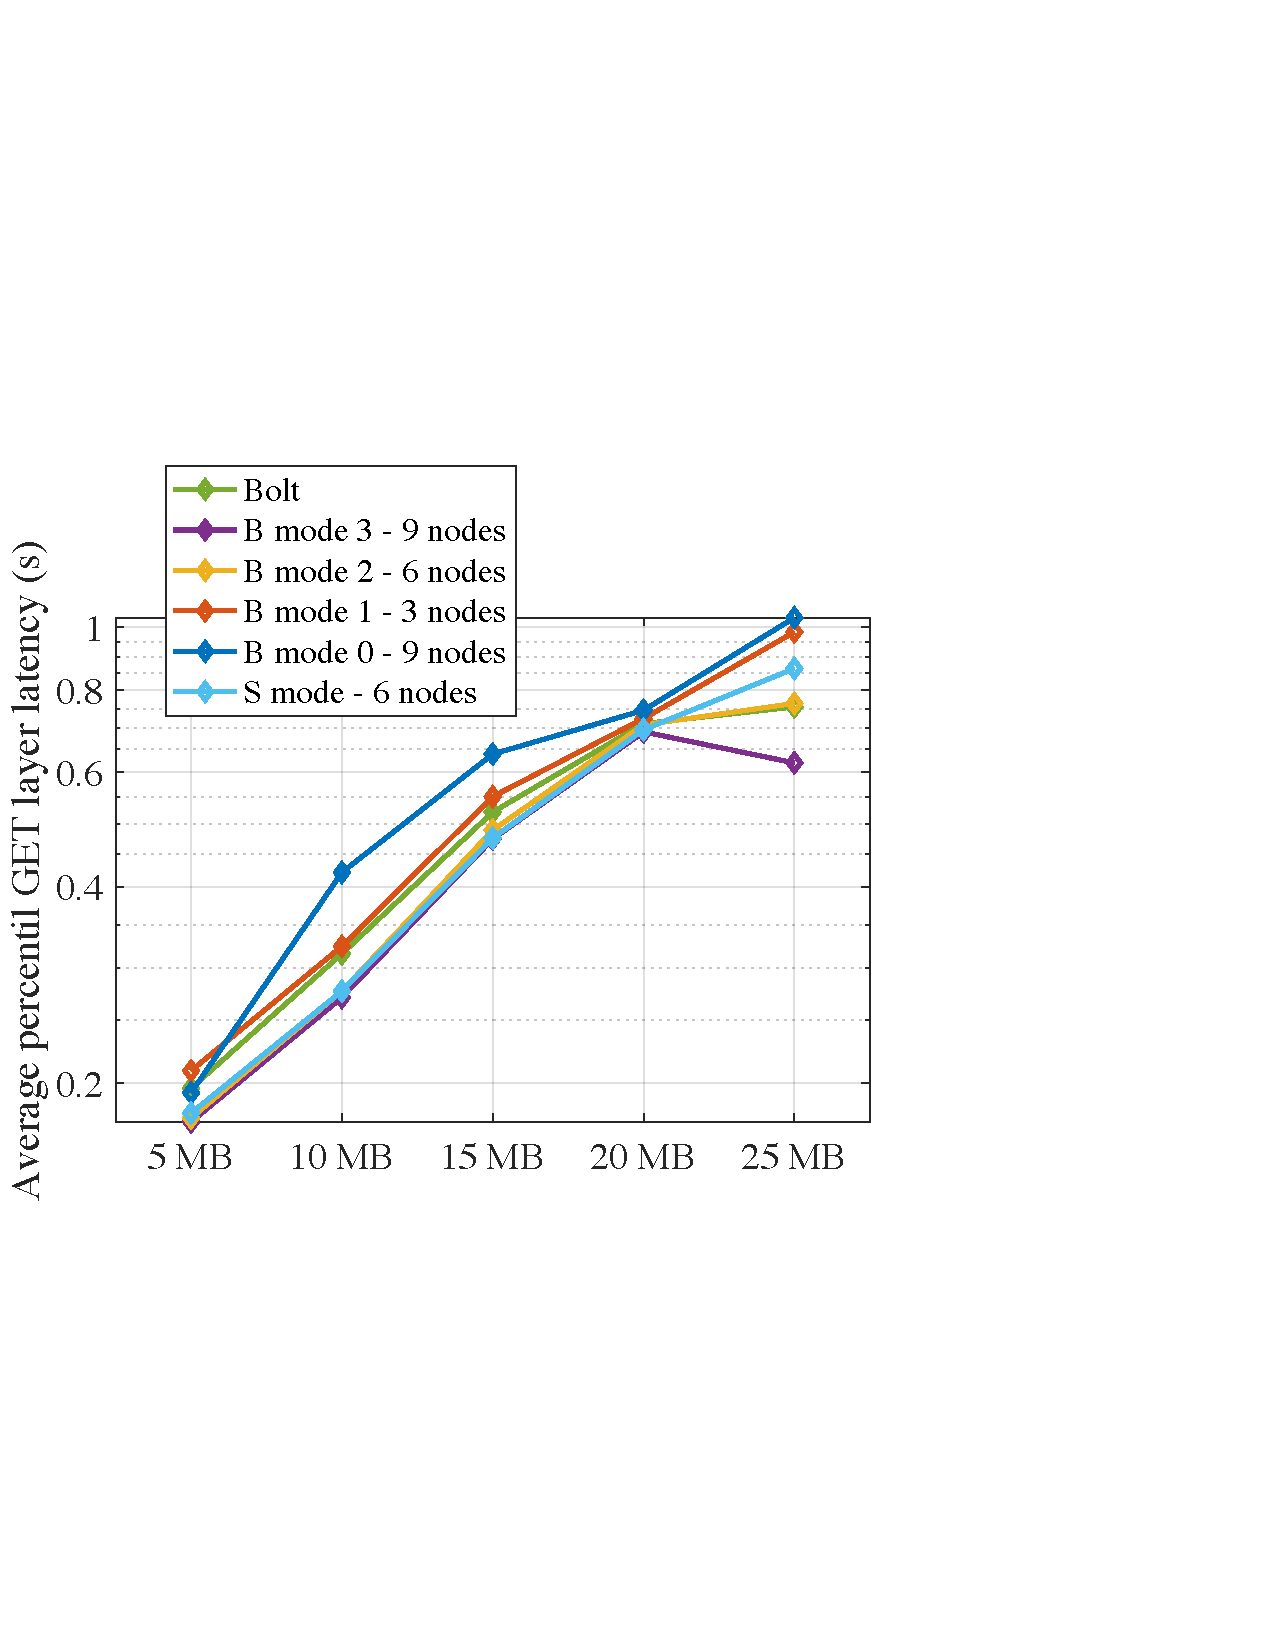
\includegraphics[width=0.9\textwidth]{graphs/dalprimaryperformance.pdf}
%		\caption{GET layer latency.\todo{add grid in background to match the other figures}}% across different schemes.}
%		\label{fig:eval-1nodegetlayerlatency}
%	\end{minipage}%
%	\begin{minipage}{0.28\textwidth}
%		\centering
%		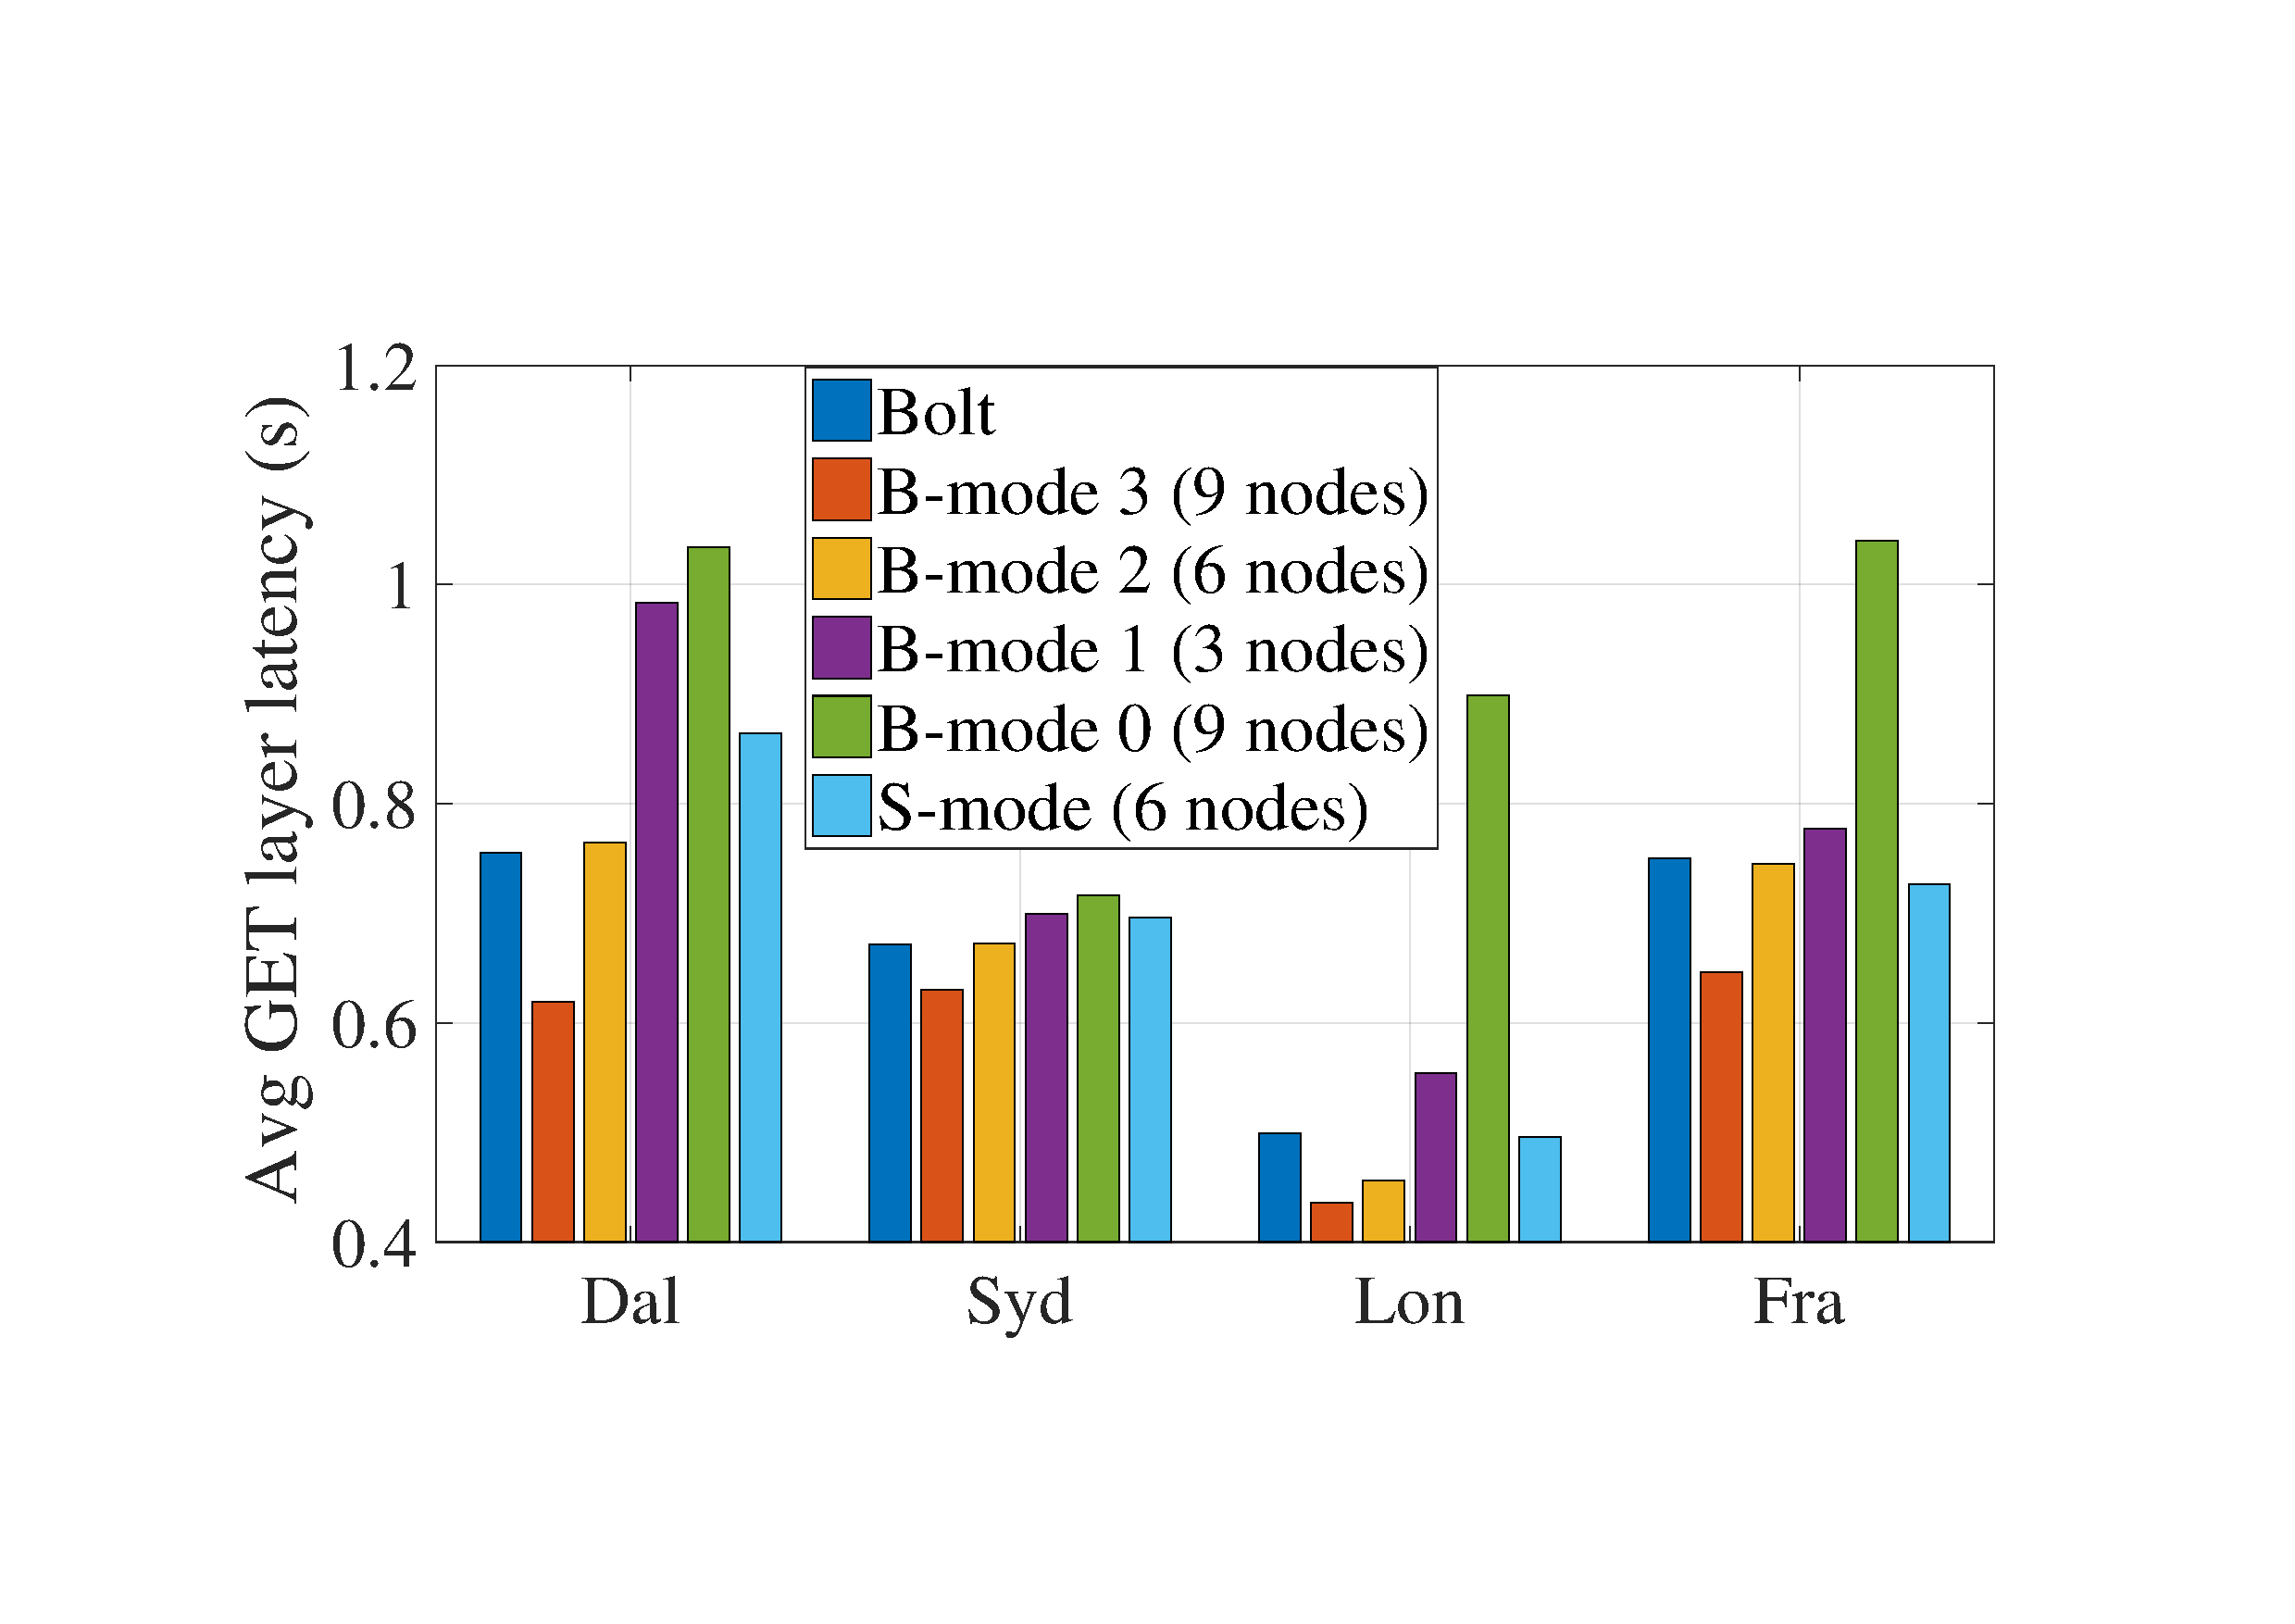
\includegraphics[width=0.9\textwidth]{graphs/total-traces.pdf}
%		\caption{Cache hit ratio.}% of LRU cache and preconstruct cache.}
%		\label{fig:eval-cachehitratios}
%	\end{minipage}%
%%	\begin{minipage}{0.3\textwidth}
%%	\centering
%%	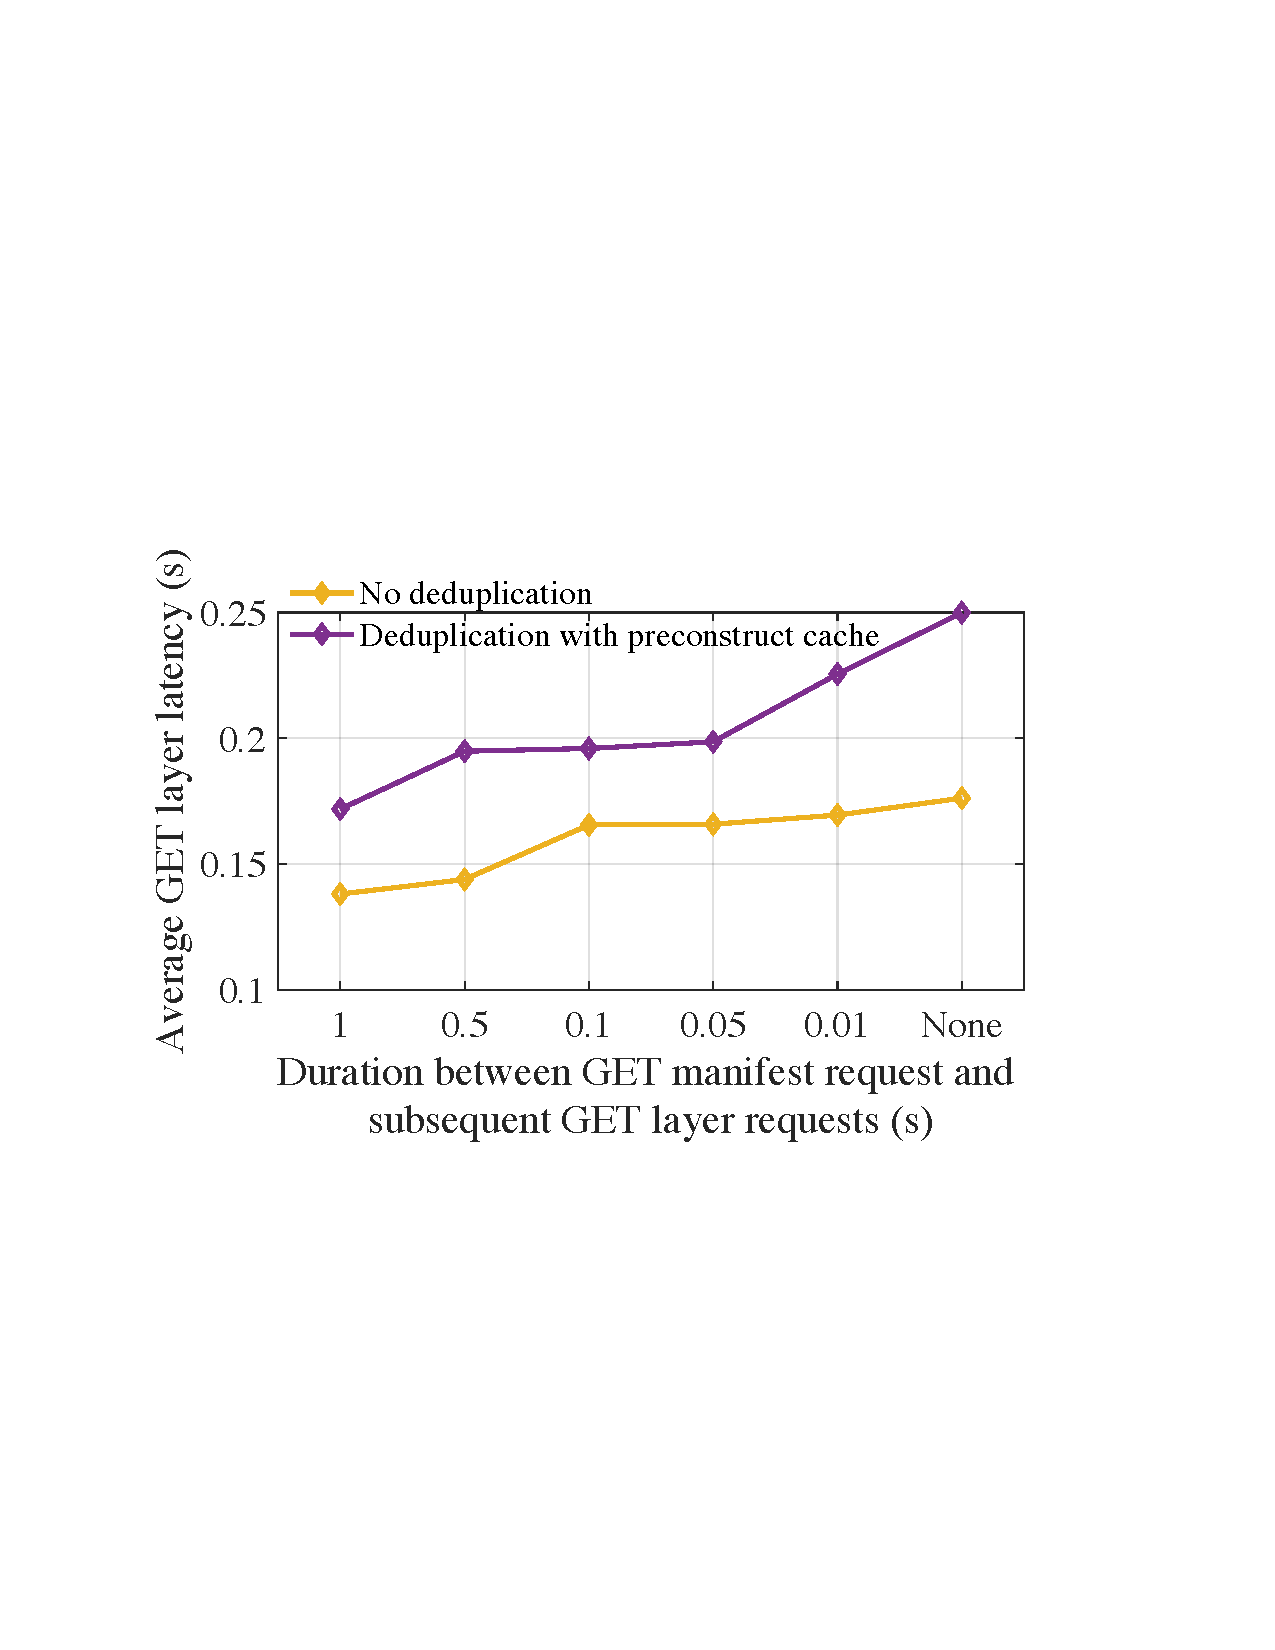
\includegraphics[width=0.9\textwidth]{graphs/durationML.pdf}
%%	\caption{The impact of durationML.}
%%	\label{fig:eval-durationML}
%%   \end{minipage}
%
%\end{figure}


\begin{figure}[t]
	\centering
	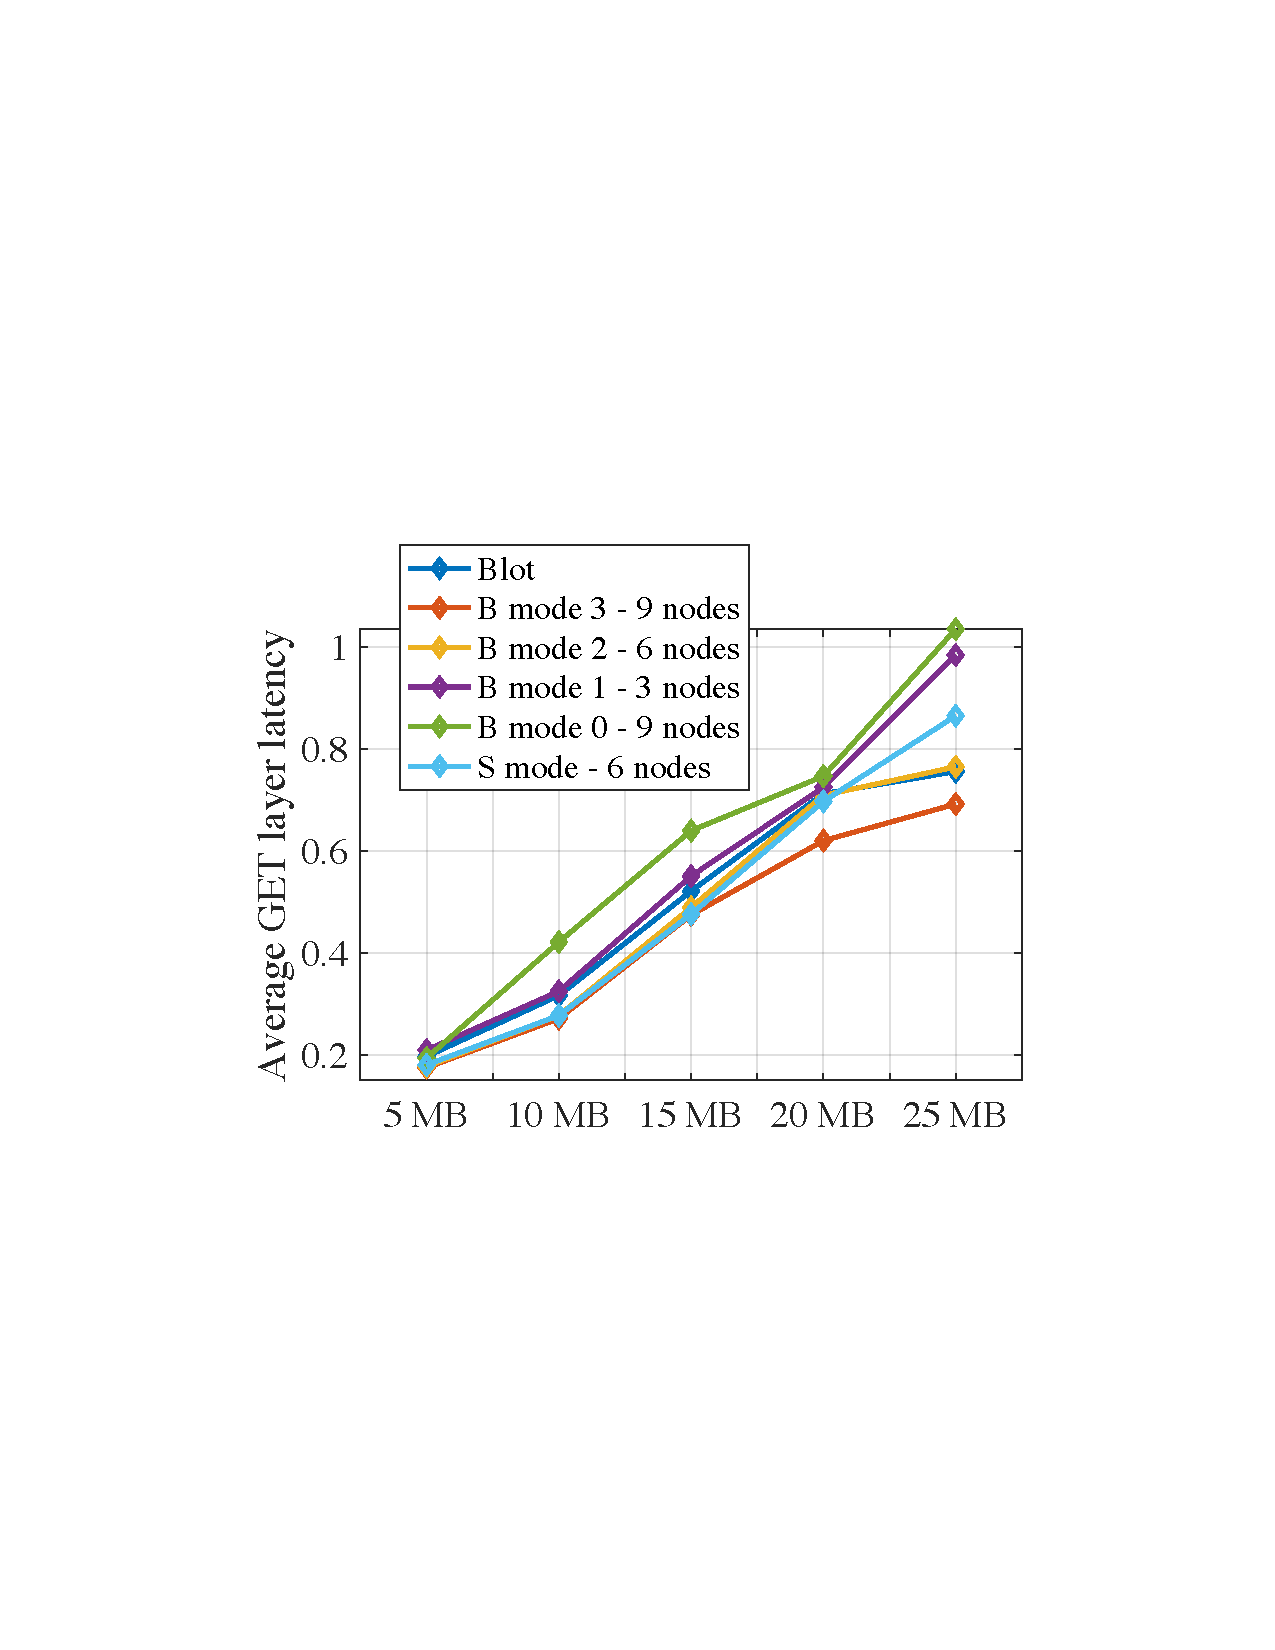
\includegraphics[width=0.3\textwidth]{graphs/dalprimary.pdf}
	\caption{Average \texttt{GET} layer latency.}
	%	\vspace{-3pt}
	\label{fig:eval-dalprimary}
	
\end{figure}

\begin{figure}[t]
	\centering
	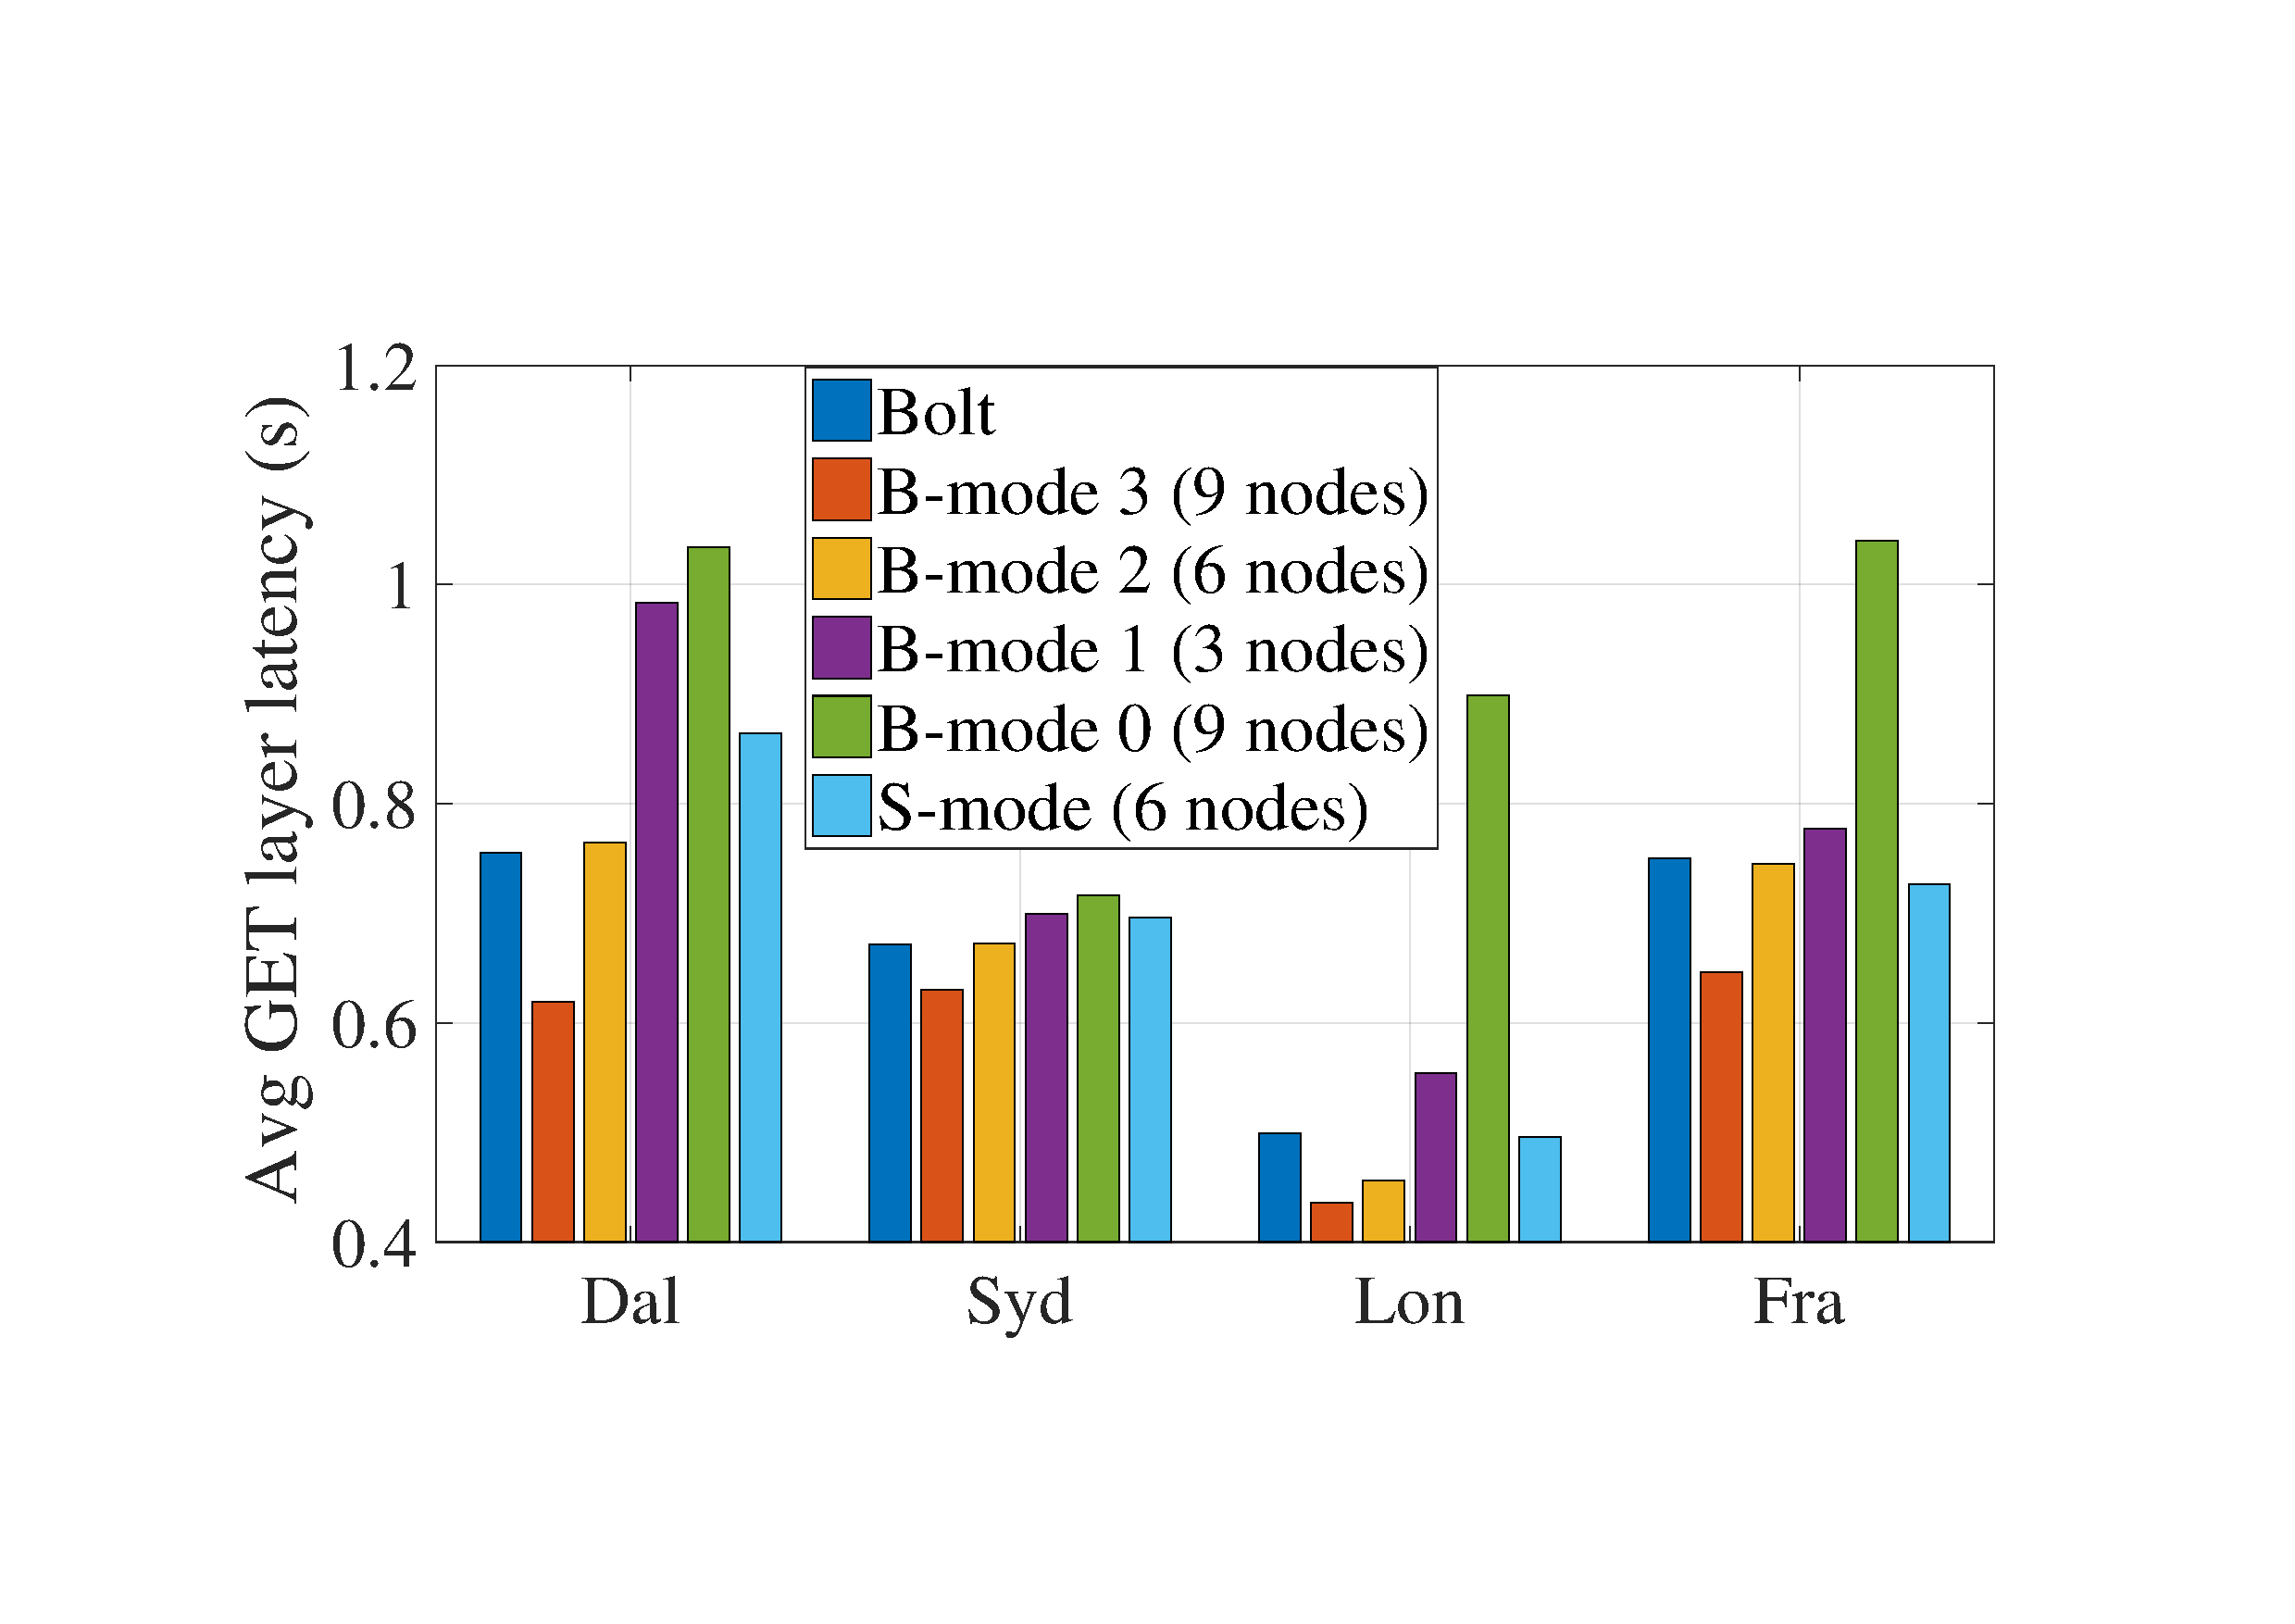
\includegraphics[width=0.3\textwidth]{graphs/total-traces.pdf}
	\caption{Average \texttt{GET} layer latency. \Subil{"Blot" in figure should be "BOLT". Why is the y axis called Average percentile GET layer latency. I don't see an explanation for that in the text}}
	%	\vspace{-3pt}
	\label{fig:eval-total-traces}
	
\end{figure}